\documentclass[tikz,border=5pt]{standalone}
\usepackage{fontspec}
\setmainfont{Times New Roman}
\usepackage{unicode-math}
\setmathfont{Cambria Math}
\usetikzlibrary{shapes.geometric,positioning,fit,backgrounds,arrows.meta,calc}

\begin{document}
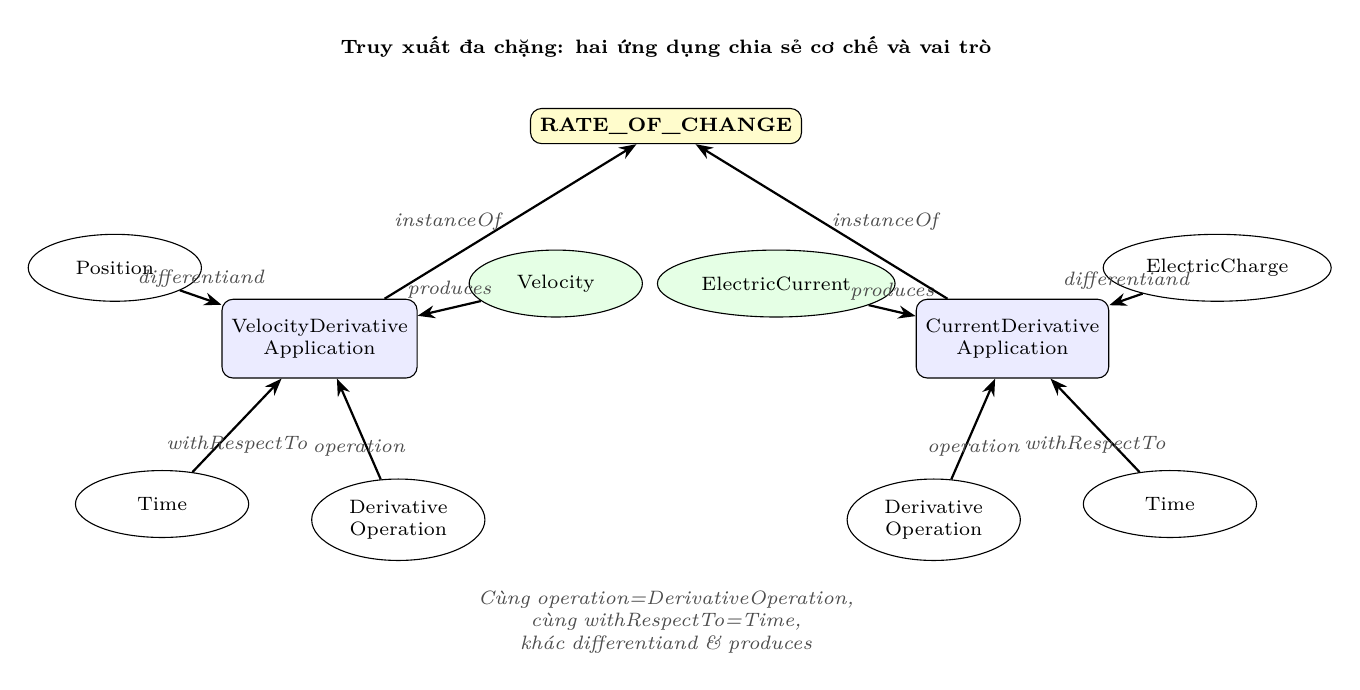
\begin{tikzpicture}[
  ent/.style={ellipse, draw, align=center, minimum width=2.2cm, minimum height=0.85cm, font=\scriptsize},
  app/.style={rectangle, draw, rounded corners, align=center, minimum height=1.0cm, font=\scriptsize},
  mech/.style={rectangle, draw, rounded corners, fill=yellow!20, align=center, font=\scriptsize\bfseries},
  arrow/.style={-{Stealth[length=2.2mm]}, thick},
  label/.style={font=\scriptsize\itshape, text=gray!60!black},
]

% === Mechanism (shared) ===
\node[mech, minimum width=3.4cm] (mech) at (0, 3.6) {RATE\_OF\_CHANGE};

% === Left application ===
\node[app, fill=blue!8] (lapp) at (-4.4, 0.9) {VelocityDerivative\\Application};
\node[ent] (ldiff) at (-7.0, 1.8) {Position};
\node[ent] (lwrt) at (-6.4, -1.2) {Time};
\node[ent] (lop)  at (-3.4, -1.4) {Derivative\\Operation};
\node[ent, fill=green!10] (lres) at (-1.4, 1.6) {Velocity};

\draw[arrow] (ldiff) -- node[label, pos=0.5, above] {differentiand} (lapp);
\draw[arrow] (lwrt)  -- node[label, pos=0.5, below] {withRespectTo} (lapp);
\draw[arrow] (lop)   -- node[label, pos=0.5, below] {operation} (lapp);
\draw[arrow] (lres)  -- node[label, pos=0.5, above] {produces} (lapp);
\draw[arrow] (lapp)  -- node[label, pos=0.5, left] {instanceOf} (mech);

% === Right application ===
\node[app, fill=blue!8] (rapp) at (4.4, 0.9) {CurrentDerivative\\Application};
\node[ent] (rdiff) at (7.0, 1.8) {ElectricCharge};
\node[ent] (rwrt) at (6.4, -1.2) {Time};
\node[ent] (rop)  at (3.4, -1.4) {Derivative\\Operation};
\node[ent, fill=green!10] (rres) at (1.4, 1.6) {ElectricCurrent};

\draw[arrow] (rdiff) -- node[label, pos=0.5, above] {differentiand} (rapp);
\draw[arrow] (rwrt)  -- node[label, pos=0.5, below] {withRespectTo} (rapp);
\draw[arrow] (rop)   -- node[label, pos=0.5, below] {operation} (rapp);
\draw[arrow] (rres)  -- node[label, pos=0.5, above] {produces} (rapp);
\draw[arrow] (rapp)  -- node[label, pos=0.5, right] {instanceOf} (mech);

% === Same roles annotation ===
\node[label, align=center, text width=5.4cm] at (0, -2.7)
  {Cùng operation=DerivativeOperation,\\cùng withRespectTo=Time,\\khác differentiand \& produces};

\node[font=\scriptsize\bfseries] at (0, 4.6) {Truy xuất đa chặng: hai ứng dụng chia sẻ cơ chế và vai trò};

\end{tikzpicture}
\end{document}